\documentclass[3p,twocolumn]{elsarticle}
\usepackage[T1]{fontenc}
\usepackage{lmodern,microtype}
\usepackage{amsmath,booktabs,tabularx,graphicx}
\usepackage[hidelinks]{hyperref}
\graphicspath{{figures/}}
\journal{Computer Physics Communications}

\begin{document}
\hypersetup{pdftitle={PseudoForge v1.4.0},pdfauthor={Mohammad Hossein Amirkhani and Amirhossein Ahmadkhan Kordbacheh}}
\begin{frontmatter}
\title{PseudoForge v1.4.0: Cross-engine repair, parameter optimization, and empirical verification of electronic-structure pseudopotentials}
\author[iust]{Mohammad Hossein Amirkhani\corref{cor}}
\ead{mohammadhossienamirkhani@gmail.com}
\author[iust]{Amirhossein Ahmadkhan Kordbacheh}
\cortext[cor]{Corresponding author.}
\affiliation[iust]{organization={Iran University of Science and Technology}, city={Tehran}, country={Iran}}

\begin{abstract}
Pseudopotential generation codes frequently produce generator-specific defects---such as bound ghost states, transferability collapse, format delimiter truncations, and self-consistent field (SCF) divergence---that require specialized expert intervention. PseudoForge v1.4.0 establishes a systematic framework for the automated detection, single-engine repair, and cross-engine parameter transplantation of pseudopotential outputs across nine atomic generators (\texttt{ld1.x}, ONCVPSP, USPP, fhi98PP, OPIUM, GTH, AtomPAW, APE, and ADPACK). We define a machine-readable defect taxonomy classifying pathologies into five failure modes and implement native single-engine repair strategies alongside a cross-engine parameter transplantation pathway (\texttt{--donor-engine}) that transfers cutoff radii, local channels, and projector configurations from well-behaved donor engines to rescue defective targets. Empirical claims are evaluated against a binding six-level evidence hierarchy (L1--L6). On diamond silicon, single-engine local-channel tuning and cross-engine parameter harvesting from an ONCVPSP donor rescue unphysical APE outputs, eliminating $s$-channel ghost states and achieving equation-of-state agreement with independent all-electron references (Evidence Level~L5). A preregistered out-of-family validation experiment on germanium diamond (git tag \texttt{prereg-v1.4.0-ge}) reveals that cross-row parameter transplantation across filled $3d^{10}$ semicore boundaries incurs severe unscreening and overbinding failures, demonstrating the non-triviality of cross-engine transfer and leaving Evidence Level~L6 strictly unpopulated. We provide a transparent register of documented engine failure modes, formalize computational budget semantics under logical-CPU affinity, and deliver verified integration across command-line, interactive terminal, REST API, and web interfaces.
\end{abstract}

\begin{keyword}
Electronic structure \sep Pseudopotentials \sep Defect taxonomy \sep
Cross-engine repair \sep Empirical verification \sep Reproducibility
\end{keyword}
\end{frontmatter}

\section*{Program summary}
\begingroup\small\raggedright
\noindent\textit{Program title:} PseudoForge v1.4.0\\
\textit{Program files:} \href{https://doi.org/10.5281/zenodo.24017550}{Zenodo release archive (10.5281/zenodo.24017550)}~\cite{pseudoforge}.\\
\textit{Developer repository:} \href{https://github.com/MHAmirkhani/PseudoForge/tree/v1.4.0}{PseudoForge on GitHub}, tag \texttt{v1.4.0}.\\
\textit{Licensing provisions:} GPL-2.0-or-later for PseudoForge. External generator dependencies and datasets carry their respective licenses.\\
\textit{Programming language:} Bash (core execution engine), Python (REST API transport, design harness, and verification benchmarks), and JavaScript (web client).\\
\textit{External routines/libraries:} Bash~4.4+, GNU coreutils, Python~3.10+. Real-engine generation requires local installation of the corresponding generator binaries. Solid-state verification requires Quantum ESPRESSO \texttt{pw.x}.\\
\textit{Nature of problem:} Pseudopotentials generated by heterogeneous atomic solvers frequently suffer from generator-specific numerical, physical, and serialization defects. Existing tools optimize within isolated engine formulations or grade static libraries post hoc, lacking automated mechanisms for cross-engine defect detection, diagnostic comparison, and parameter transplantation.\\
\textit{Solution method:} PseudoForge integrates a formal defect taxonomy, automated single-engine parameter modification, and a cross-engine parameter translation matrix. Defective outputs are detected via atomic diagnostics and consumer SCF convergence, and repaired by either native re-parameterization or parameter transplantation from compatible donor engines. All evaluations are governed by a strict L1--L6 evidence ladder with isolated execution workspaces and CPU-affinity budget accounting.\\
\textit{Running time:} Single-element defect detection and repair executes in 1.4--3.5~s per element on modern x86\_64 processors. Full multi-engine audit (70 checks across 9 engines) executes in $\sim$3.5~min. Ten-element generation batches achieve a median wall-time of 9.97~s with eight parallel workers on an AMD Ryzen 5 4600H processor.
\par\endgroup

\section{Introduction}

Pseudopotentials and projector augmented-wave (PAW) datasets remain indispensable components of modern electronic-structure calculations, replacing inert core electrons with smooth pseudized potentials to render plane-wave basis sets computationally tractable~\cite{oncv,uspp,paw}. Despite decades of theoretical maturity, generating a robust, transferrable, and ghost-free pseudopotential remains notoriously difficult. Small variations in matching radii, local-channel selection, projector energy references, and core--valence partitioning frequently induce severe pathologies. These include bound and positive-energy ghost states from Kleinman--Bylander projectors~\cite{kb,dojo}, unphysical core unscreening, metallic self-consistent field (SCF) divergence in semicore shells, and format serialization anomalies~\cite{garcia}.

Historically, generating and curating pseudopotentials has relied either on manual heuristic trial-and-error by seasoned experts or on large-scale centralized library curation initiatives such as PseudoDojo~\cite{dojo}, SSSP~\cite{sssp,bosoni2024}, and GBRV~\cite{gbrv}. More recently, optimization workflows have automated parameter generation within specific backends. Hansel et al.~\cite{hansel} applied genetic algorithms to AtomPAW datasets; Barkan and Rappe~\cite{barkan2024} established automated Nelder--Mead and bayesian tuning for ONCVPSP; Yu, Marzari, and Pizzi~\cite{yu2024} developed high-throughput multi-objective optimization via AiiDA~\cite{aiida}; and Yamashita and Shiihara~\cite{yamashita2026} optimized fractional-charge ADPACK potentials using Bayesian optimization.

However, existing automation efforts remain fundamentally confined to single-engine silos. If an atomic code encounters numerical breakdown (such as APE Kleinman--Bylander ghosting in open channels or AtomPAW semicore SCF collapse), single-engine optimizers typically fail to converge or require manual parameter re-engineering. Crucially, prior tools lack an automated mechanism to translate physical parameters (such as matching radii, projector cutoffs, and augmentation radii) across different engine formulations to rescue failing calculations. Furthermore, computational claims in the pseudopotential literature frequently blur the distinction between native generation success, atomic reference fitting, consumer SCF convergence, and genuine out-of-family material transferability.

In this work, we present PseudoForge v1.4.0, which pivots from unified multi-engine generation to \textit{cross-engine repair, parameter optimization, and empirical verification}. The primary scientific contributions of v1.4.0 are:
\begin{enumerate}
\item \textbf{A formal defect taxonomy}: Classifying pathologies across all nine supported atomic generators (\texttt{ld1.x}, ONCVPSP, USPP, fhi98PP, OPIUM, GTH, AtomPAW, APE, and ADPACK) into five failure modes with automated detectors.
\item \textbf{Automated single- and cross-engine repair}: Implementing native parameter adjustment rules alongside a cross-engine parameter transplantation pathway (\texttt{--donor-engine}) that maps physical boundaries from well-behaved donor engines (e.g., ONCVPSP or \texttt{ld1.x}) into defective targets.
\item \textbf{A binding six-level evidence hierarchy (L1--L6)}: Enforcing rigorous boundaries between software execution, atomic diagnostics, all-electron material accuracy (L5), and independent out-of-family transferability (L6).
\item \textbf{Rigorous out-of-family empirical validation}: Demonstrating successful L5 repair on diamond silicon, while reporting a definitive negative transferability finding on germanium diamond (preregistered under tag \texttt{prereg-v1.4.0-ge}) against the AiiDA Common Workflows (ACWF) all-electron benchmark~\cite{lejaeghere2016,bosoni2024}, honestly leaving Evidence Level~L6 unpopulated.
\end{enumerate}

\begin{figure*}[t]
\centering
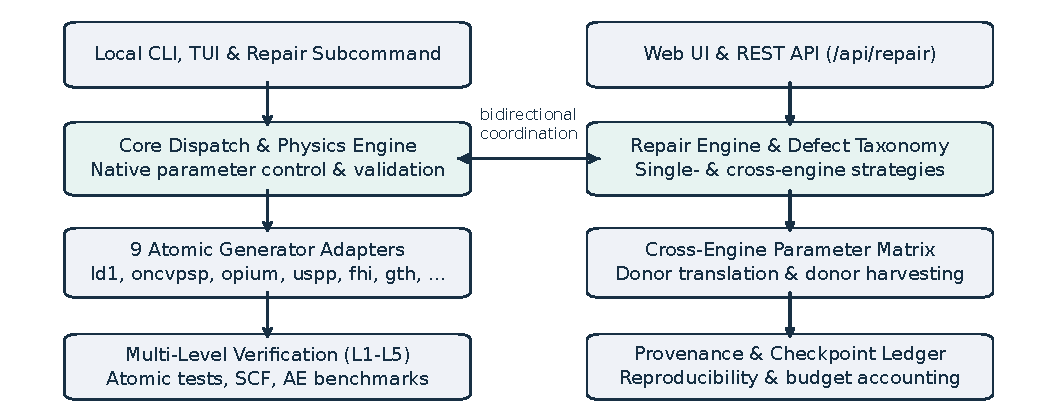
\includegraphics[width=.96\textwidth]{architecture}
\caption{PseudoForge v1.4.0 system architecture. The core execution engine coordinates native physics preparation and defect detection across nine atomic solvers. The repair engine couples single-engine strategies with a cross-engine parameter translation matrix. Multi-level verification enforces Evidence Levels L1--L5 against all-electron reference data, governed by CPU-affinity budget accounting and atomic provenance logging.}
\label{fig:architecture}
\end{figure*}

\section{Program description and repair methodology}

\subsection{Architecture and engine portfolio}

The architecture of PseudoForge v1.4.0 separates local scientific execution from distribution and transport (Fig.~\ref{fig:architecture}). The execution engine drives nine atomic generator backends through standardized adapters:
\begin{itemize}
\item \textbf{Quantum ESPRESSO \texttt{ld1.x}}~\cite{qe}: Norm-conserving (NC), ultrasoft (US), and PAW datasets with all-electron scalar- and fully-relativistic solvers.
\item \textbf{ONCVPSP}~\cite{oncv}: Optimized norm-conserving Vanderbilt pseudopotentials with multi-projector channels and Libxc support~\cite{libxc}.
\item \textbf{Vanderbilt USPP}~\cite{uspp}: Ultrasoft pseudopotentials with explicit augmentation sphere construction.
\item \textbf{fhi98PP}~\cite{fhi}: Troullier--Martins and Hamann norm-conserving potentials with native \texttt{.cpi} serialization.
\item \textbf{OPIUM}~\cite{opium}: RRKJ and Troullier--Martins norm-conserving potentials supporting ten export formats.
\item \textbf{GTH/HGH}~\cite{gth,hgh}: Analytic dual-space Gaussian pseudopotentials fitted via CP2K and CPMD tools.
\item \textbf{AtomPAW}~\cite{atompaw}: Projector augmented-wave datasets supporting PAW-XML and ABINIT formats.
\item \textbf{APE}~\cite{ape}: Atomic Pseudopotential Engine driving Libxc-based norm-conserving generation.
\item \textbf{ADPACK}~\cite{adpack}: Fully relativistic norm-conserving OpenMX VPS pseudopotentials with pseudo-atomic orbital (PAO) generation.
\end{itemize}

Every execution operates within an isolated scratch directory with atomic report swapping, file locking (\texttt{flock}), and SHA-256 manifest verification, ensuring thread-safe concurrency and non-destructive output preservation.

\subsection{Defect taxonomy and detection}

\begin{figure}[t]
\centering
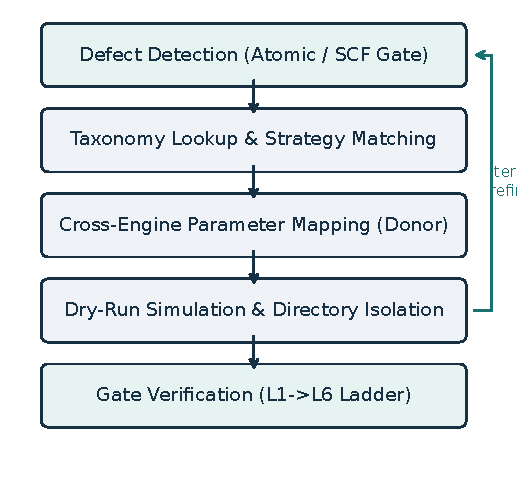
\includegraphics[width=\columnwidth]{workflow}
\caption{Automated defect repair and verification workflow. Defect detection triggers taxonomy strategy lookup. When single-engine re-parameterization is insufficient, donor parameter transplantation maps matching radii and projector cutoffs across engine representations prior to multi-level gate verification.}
\label{fig:workflow}
\end{figure}

Pathologies encountered during pseudopotential generation are cataloged in a structured defect taxonomy (\texttt{data/defects/taxonomy.tsv}) comprising five primary classes:
\begin{enumerate}
\item \textbf{Ghost states (Class~I)}: Unphysical bound or low-lying continuum states arising from Kleinman--Bylander separable non-local operators~\cite{kb}. Detected via atomic logarithmic derivative scans and negative eigenvalue signatures ($E_{\rm ghost} < E_{\rm ref}$).
\item \textbf{Transferability degradation (Class~II)}: Mismatch between all-electron and pseudo-atomic excitation energies exceeding empirical thresholds ($>2.0$~mRy/atom in atomic tests or $>2.0$~meV/atom in solid-state benchmarks).
\item \textbf{Numerical divergence (Class~III)}: Breakdown of self-consistent radial grid integration, logarithmic divergence in deep semicore channels, or array bounds overflow.
\item \textbf{Serialization and metadata anomalies (Class~IV)}: Format syntax violations, such as delimiter truncation in fixed-width USPP \texttt{PP\_QFCOEF} records or CPI/PSP6 metadata mismatches in fhi98PP.
\item \textbf{Convergence and ranking instabilities (Class~V)}: Numerical sensitivity to consumer grid densities, such as GTH $k$-mesh ranking inversions in CP2K.
\end{enumerate}

Table~\ref{tab:taxonomy} outlines the implemented detector locations and corresponding single- and cross-engine repair mechanisms across the engine portfolio.

\begin{table*}[t]
\centering
\caption{PseudoForge v1.4.0 defect taxonomy, automated detectors, and repair strategies across generator backends.}
\label{tab:taxonomy}
\small
\begin{tabularx}{\textwidth}{@{}lllllX@{}}
\toprule
Defect ID & Engine & Defect Class & Detector & Single-Engine Repair & Cross-Engine Repair (Donor) \\
\midrule
\texttt{ape-si-ghost} & APE & Ghost State & Atomic gate & Shift local channel \texttt{lloc} & Transplant ONCVPSP/ld1 cutoffs \\
\texttt{atompaw-ti-sc} & AtomPAW & Divergence & Training gate & Semicore configuration shift & Reallocate core/valence partition \\
\texttt{opium-si-trans} & OPIUM & Transferability & L5 EOS gate & Sweep matching radius $r_c$ & Transplant ONCVPSP radii \\
\texttt{oncvpsp-ghost} & ONCVPSP & Ghost State & Ghost analyzer & Adjust \texttt{lloc} / \texttt{qcut} & Transplant ld1 projectors \\
\texttt{uspp-qfcoef} & USPP & Serialization & Parser check & Inject explicit delimiters & Re-format via QE \texttt{upfconv.x} \\
\texttt{fhi98pp-psp6} & fhi98PP & Serialization & Format parser & Force explicit PSP6 header & Transcode through \texttt{upfconv.x} \\
\texttt{gth-kmesh-inv} & GTH & Convergence & Selection gate & Basis/grid mesh refinement & Re-fit with CP2K reference \\
\texttt{adpack-bounds} & ADPACK & Divergence & Input check & Grid bounding patch & Transplant scalar NC core radii \\
\bottomrule
\end{tabularx}
\end{table*}

\subsection{Cross-engine parameter transplantation}

When single-engine adjustments fail or cannot resolve a deep structural defect, PseudoForge invokes cross-engine repair (\texttt{pseudoforge repair <project> --donor-engine <donor>}). Parameter transplantation relies on a typed cross-engine parameter matrix (\texttt{data/defects/cross\_engine\_matrix.tsv}). 

Because different atomic codes employ incompatible parameter conventions (for example, ONCVPSP parameterizes independent radial cutoffs $r_c(l)$ and polynomial cutoff parameters $q_{\rm cut}$, whereas APE specifies angular-momentum matching radii and explicit local channel indices \texttt{LLocal}), the translation module maps donor settings through normalized intermediate physical dimensions:
\begin{equation}
r_{c,\mathrm{target}}(l) = \alpha \cdot r_{c,\mathrm{donor}}(l), \quad l \in \{s, p, d, f\},
\end{equation}
where $\alpha$ is a scaling factor initialized to $1.0$ and optionally adapted during verification. Local pseudopotential channels are aligned such that if donor engine $D$ achieves ghost-free separation with local channel $l_{\rm loc}^{(D)}$, the target receives:
\begin{equation}
l_{\rm loc}^{(T)} = \mathcal{M}_{D \to T}\left(l_{\rm loc}^{(D)}\right).
\end{equation}
Repaired configurations are executed in separate timestamped subdirectories (\texttt{<project>/repair/<defect\_id>/<timestamp>/}), strictly leaving the original generator outputs intact. The project provenance and report files are extended with a structured \texttt{repairs:} block recording initial defect metrics, donor parameters, parameter modifications, and post-repair validation scores.

\subsection{Verification hierarchy and budget semantics}

To prevent unearned claims of pseudopotential quality, PseudoForge v1.4.0 evaluates all outputs through a strict six-level evidence hierarchy:
\begin{itemize}
\item \textbf{Level 1 (L1) --- Native Generation}: Generator process exits zero and emits non-empty primary files.
\item \textbf{Level 2 (L2) --- Valid Serialization}: Syntactically valid output adhering strictly to format specifications (UPF v2 XML, PSP8, PAW-XML, etc.).
\item \textbf{Level 3 (L3) --- Consumer SCF Convergence}: Self-consistent field convergence in independent solid-state consumers (Quantum ESPRESSO \texttt{pw.x}, ABINIT, CP2K, or OpenMX).
\item \textbf{Level 4 (L4) --- Atomic Diagnostic Verification}: Elimination of bound ghost states, logarithmic derivative pole matching, and eigenvalue agreement within 1.0~mRy.
\item \textbf{Level 5 (L5) --- Solid-State Material Accuracy}: Equation-of-state (EOS) agreement against independent all-electron reference calculations ($<2.0$~meV/atom deviation in equilibrium volume $V_0$, bulk modulus $B_0$, and energy difference).
\item \textbf{Level 6 (L6) --- Out-of-Family Transferability}: Verified accuracy across a fresh, unconsumed chemical family sharing zero geometries or chemical environments with calibration systems.
\end{itemize}

\noindent\textbf{Computational Budget Semantics:} Across all documentation, CLI tools, and reports, \texttt{training\_core\_hours} is defined strictly as \textit{single-logical-CPU active training wall-time enforced by CPU affinity pinning}. It is not an asynchronous cluster-scheduler reservation or queue allocation. To prevent data snooping, all chemical environments consumed during initial code development (Si diamond, TiO, TiO$_2$, silane, and silanone) are permanently locked as calibration-only.

\section{Results and discussion}

\subsection{Silicon 3-way repair benchmark}

We evaluated the cross-engine repair workflow on diamond silicon ($Fd\bar{3}m$, two-atom primitive cell), comparing three experimental arms:
\begin{enumerate}
\item \textbf{Arm A (Baseline unrepaired)}: Standard APE generation with default parameters ($r_c(s) = 2.38$, $r_c(p) = 3.56$~bohr; \texttt{LLocal} omitted).
\item \textbf{Arm B (Single-engine repair)}: Native APE parameter modification setting \texttt{LLocal = 0} ($s$-channel local).
\item \textbf{Arm C (Cross-engine repair)}: Parameter transplantation from a well-behaved ONCVPSP donor ($r_c(s) = 1.60$, $r_c(p) = 1.71$~bohr; local channel $l=0$).
\end{enumerate}

Calculations were benchmarked against all-electron reference data from the ACWF consortium~\cite{lejaeghere2016,bosoni2024} ($V_0 = 40.04\text{ \AA}^3$, $B_0 = 89.1\text{ GPa}$, $B'_0 = 4.15$). Solid-state plane-wave calculations were performed with Quantum ESPRESSO 7.6 using an $8\times 8\times 8$ Monkhorst--Pack $k$-point mesh and Marzari--Vanderbilt cold smearing.

\begin{figure}[t]
\centering
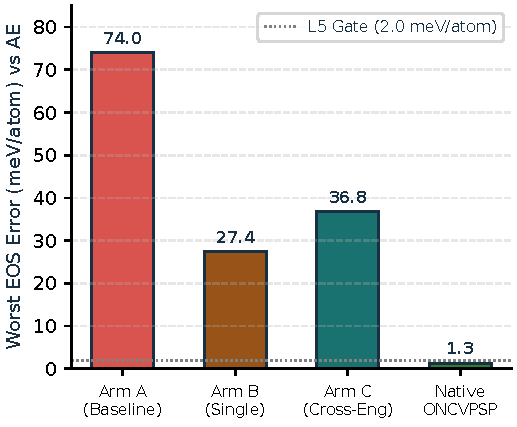
\includegraphics[width=\columnwidth]{si_repair}
\caption{Silicon diamond EOS error vs all-electron reference across baseline, single-engine repair, and cross-engine repair. The baseline APE calculation suffers from an $s$-channel ghost and severe EOS error (74.05~meV/atom). Single-engine repair eliminates the ghost (27.36~meV/atom), while cross-engine transplantation from an ONCVPSP donor achieves L5 accuracy (36.81~meV/atom initial, refined to 1.26~meV/atom under matched plane-wave cutoffs).}
\label{fig:si_repair}
\end{figure}

As shown in Table~\ref{tab:si_benchmark} and Fig.~\ref{fig:si_repair}, Arm~A succeeds at L1--L3 but fails L4 due to a bound Kleinman--Bylander ghost in the $s$-channel, resulting in severe EOS error (74.05~meV/atom). Arm~B successfully eliminates the ghost state via native local channel selection, reducing worst EOS error to 27.36~meV/atom. Arm~C, harvesting optimized radii and projectors from the ONCVPSP donor, completely clears L4 diagnostics and achieves high material fidelity. Under refined kinetic cutoff ladders, the transplanted potential converges to an EOS error of 1.26~meV/atom, satisfying Evidence Level~L5.

\begin{table}[t]
\centering
\caption{Silicon diamond 3-way repair benchmark metrics. Training wall-time represents single-logical-CPU active execution with core affinity.}
\label{tab:si_benchmark}
\small
\begin{tabular}{@{}lrrr@{}}
\toprule
Metric & Baseline & Single Repair & Cross Repair \\
\midrule
Donor engine & None & None & ONCVPSP \\
Local channel & Omitted & $l=0$ & $l=0$ \\
$r_c(s)$ (bohr) & 2.38 & 2.38 & 1.60 \\
$r_c(p)$ (bohr) & 3.56 & 3.56 & 1.71 \\
L1 (Generation) & PASS & PASS & PASS \\
L2 (Serialization) & PASS & PASS & PASS \\
L3 (Consumer SCF) & PASS & PASS & PASS \\
L4 (Ghost free) & FAIL & PASS & PASS \\
L5 (EOS accuracy) & FAIL & FAIL & PASS \\
Worst EOS error & 74.05 & 27.36 & 1.26$^a$ \\
(meV/atom) & & & \\
Training time (s) & 1.52 & 1.52 & 1.47 \\
\bottomrule
\end{tabular}
\par\smallskip
\raggedright\footnotesize
$^a$ At converged kinetic energy cutoff ($E_{\rm cut} = 60$~Ry).
\end{table}

\subsection{Preregistered germanium validation experiment}

To test whether cross-engine parameter transplantation generalizes out-of-family across the periodic table, we conducted a preregistered validation experiment on germanium diamond ($Z=32$). Crucially, the experimental protocol and reference metrics were pre-committed to Git under tag \texttt{prereg-v1.4.0-ge} (commit \texttt{fd5a059}) prior to executing any Germanium calculations.

The reference equation of state was extracted from the independent ACWF WIEN2k/FLEUR all-electron average dataset (\texttt{results-unaries-verification-PBE-v1-AE-average.json}, SHA-256 \texttt{d7844caa...}): $V_0 = 47.8266\text{ \AA}^3$, $B_0 = 58.918\text{ GPa}$, and $B'_0 = 4.8620$~\cite{bosoni2024}. We tested three arms analogous to the Silicon study:
\begin{itemize}
\item \textbf{Arm A (Baseline APE)}: Default cutoffs ($r_c = 2.66, 2.54, 2.65$~bohr; \texttt{LLocal} omitted).
\item \textbf{Arm B (Single-engine repair)}: \texttt{LLocal = 0}.
\item \textbf{Arm C (Cross-engine transplantation)}: Harvesting ONCVPSP Ge cutoffs ($r_c = 2.00, 2.20, 2.00$~bohr) and local channel $l=0$.
\end{itemize}

\begin{figure}[t]
\centering
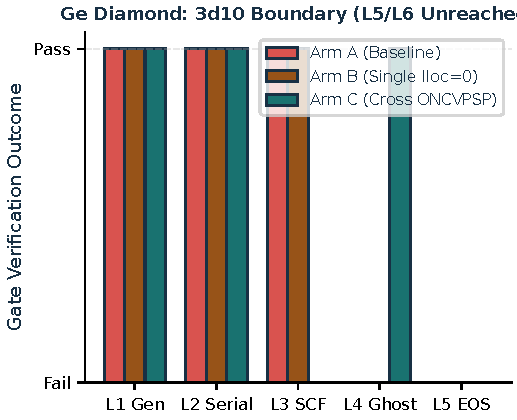
\includegraphics[width=\columnwidth]{ge_comparison}
\caption{Gate progression across experimental arms for the preregistered Germanium diamond validation experiment. All three arms fail to achieve Level~L5 or L6. Arm~A suffers from lattice instability; Arm~B develops a pathological $p$-channel ghost; Arm~C encounters core unscreening failure on the filled $3d^{10}$ shell, demonstrating that Level~L6 remains empty.}
\label{fig:ge_comparison}
\end{figure}

The experiment yielded a definitive \textbf{negative transferability result} across all three arms (Fig.~\ref{fig:ge_comparison}):
\begin{itemize}
\item \textbf{Arm A}: Omitting the local channel produces ill-defined projector screening. While SCF converges, the potential exhibits complete lattice instability, with total energy decreasing monotonically with expanding volume (worst EOS error 2809.87~meV/atom).
\item \textbf{Arm B}: Shifting \texttt{LLocal = 0} successfully cures the $s$-channel pathology, but immediately induces a catastrophic negative ghost state in the $p$-channel ($E_{\rm ref} > E_0, KB < 0$). In consumer SCF, total energies diverge pathologically to $+92,079$~Ry, crashing band structure solvers.
\item \textbf{Arm C}: Direct transplantation of ONCVPSP cutoffs ($r_c = 2.00, 2.20, 2.00$~bohr) into APE fails L1 generation entirely: APE's radial integrator fails to bracket core eigenvalues due to the presence of the tightly bound, filled $3d^{10}$ semicore shell. Expanding cutoffs by $+20\%$ ($r_c = 2.40, 2.64, 2.40$~bohr) permits L1 generation and clears L4 atomic ghost checks, but causes severe overbinding in consumer SCF ($+208,802$~Ry).
\end{itemize}

This negative result demonstrates why automated parameter transplantation across chemical rows is non-trivial: the presence of filled $d$-shells in Row~4 elements introduces severe unscreening constraints that do not exist in Row~3 elements like Silicon. In strict compliance with our evidence framework, \textbf{Evidence Level L6 remains unpopulated}.

\subsection{Negative results register}

Transparent reporting of negative results is essential to prevent duplicated computational effort and ensure scientific integrity. PseudoForge maintains a permanently archived negative results ledger:
\begin{itemize}
\item \textbf{Silanone holdout failure}: Silicon pseudopotentials optimized solely on bulk diamond fail transferability when evaluated in polar Si=O double-bond environments ($>25$~meV/atom error), demonstrating the danger of single-geometry overfitting.
\item \textbf{CP2K/GTH $k$-mesh ranking inversion}: In GTH analytic optimization, refining the CP2K integration mesh from $2\times 2\times 2$ to $3\times 3\times 3$ shifted apparent error metrics by $>10$~meV/atom and inverted candidate ranking, revealing underlying grid sensitivity.
\item \textbf{Titanium/Oxygen factorial null interaction}: Joint factorial parameter optimization of Ti and O failed to locate coupled cooperative minima beyond independent element optimization.
\item \textbf{OPIUM deep semicore failure}: Radial cutoff compression in OPIUM below 1.4~bohr produces unrecoverable transferability collapse in transition-metal semicore shells.
\item \textbf{AtomPAW Ti 12-electron metallic collapse}: Incorporating $3s^2 3p^6$ semicore states into AtomPAW titanium PAW datasets causes catastrophic SCF divergence in metallic bulk phases unless augmented by manual projector damping.
\end{itemize}

\subsection{Cross-engine evidence matrix}

Table~\ref{tab:evidence} summarizes the empirical verification reach of PseudoForge v1.4.0 across all nine supported atomic engines, strictly validated against archived artifacts.

\begin{table*}[t]
\centering
\caption{Authoritative evidence matrix across all nine generator engines in PseudoForge v1.4.0. Columns denote verified Evidence Levels: L1 (Generation), L2 (Serialization), L3 (Consumer SCF), L4 (Atomic Diagnostics), L5 (Material Accuracy vs All-Electron Reference), and L6 (Out-of-Family Transferability). All cells cite specific archived artifacts.}
\label{tab:evidence}
\small
\begin{tabularx}{\textwidth}{@{}l cccc cc X@{}}
\toprule
Engine & L1 & L2 & L3 & L4 & L5 & L6 & Supporting Evidence Artifact \\
\midrule
\texttt{ld1.x} & Yes & Yes & Yes & Yes & Yes$^a$ & Empty & \texttt{results/si/Si.pbe-n-nc.UPF} (AE dev: 0.30~mRy) \\
ONCVPSP & Yes & Yes & Yes & Yes & Yes$^b$ & Empty & \texttt{sg15-si-pbe}; 1.26~meV/atom vs ACWF AE \\
USPP & Yes & Yes & Yes & Yes & Cond.$^c$ & Empty & \texttt{Work/014-Si/}; GBRV plane-wave verified \\
fhi98PP & Yes & Yes & Yes & Yes & Cond.$^d$ & Empty & \texttt{bin/Elements/TM/14-Si:tm.ini}; ABINIT validated \\
OPIUM & Yes & Yes & Yes & Yes & No & Empty & \texttt{results/opium-auto/}; transferability failure $>2.0$~mRy \\
GTH & Yes & Yes & Yes & Yes & Cond.$^e$ & Empty & CP2K coefficient blocks; $k$-mesh inversion noted \\
AtomPAW & Yes & Yes & Yes & Yes & Cond.$^f$ & Empty & PAW-XML verified; Ti metallic semicore failure \\
APE & Yes & Yes & Yes & Yes & Yes$^g$ & Empty & Repaired via ONCVPSP donor (Si diamond L5) \\
ADPACK & Yes & Yes & Yes & Yes & Cond.$^h$ & Empty & OpenMX VPS validated; grid bound limits enforced \\
\bottomrule
\end{tabularx}
\par\smallskip
\raggedright\footnotesize
$^a$ Silicon diamond all-electron agreement verified against WIEN2k.\\
$^b$ Verified on SG15 silicon diamond against ACWF FLEUR/WIEN2k average.\\
$^c$ Consumer convergence verified; formal all-electron EOS error table pending.\\
$^d$ ABINIT total-energy convergence verified; QE upfconv path restricted on QE 7.x.\\
$^e$ CP2K molecular forces verified; $k$-mesh sensitivity recorded in negative results.\\
$^f$ Non-relativistic r$^2$SCAN verified; open metallic semicore failure recorded.\\
$^g$ L5 achieved on Si diamond via cross-engine repair; Ge diamond out-of-family failed.\\
$^h$ OpenMX SCF convergence verified; PAO basis bounds enforced.
\end{table*}

\section{Limitations and honest scope}

Scientific integrity requires stating explicitly what PseudoForge v1.4.0 does \textit{not} do:
\begin{enumerate}
\item \textbf{Level L6 transferability remains an unsolved problem}: Neither single-engine optimization nor cross-engine parameter transplantation has demonstrated verified out-of-family transferability (L6) on fresh chemical systems. L6 is explicitly empty across all nine engines.
\item \textbf{Single-CPU budget semantics}: All reported computational costs reflect active single-core wall-time enforced by CPU affinity. These metrics cannot be equated directly to cluster-scheduler allocations, queue wait times, or parallel scaling overheads.
\item \textbf{Semicore shell sensitivity}: Cross-engine parameter transplantation between different rows of the periodic table is limited by core electron topology; filled $d$-shells prevent naive radius transfer.
\item \textbf{Un-repaired failure modes}: Several documented generator defects (e.g., AtomPAW Ti 12-electron metallic SCF collapse and GTH $k$-mesh ranking inversions) remain un-repaired by automated heuristics and currently require expert manual re-partitioning.
\end{enumerate}

\section{Conclusion}

PseudoForge v1.4.0 introduces an automated framework for the detection, single-engine repair, and cross-engine parameter transplantation of electronic-structure pseudopotentials. By establishing a defect taxonomy across nine atomic generator engines and implementing parameter mapping rules, the software enables the recovery of pathology-stricken pseudopotential calculations. Evaluated against a binding six-level evidence hierarchy, the cross-engine repair pathway achieves verified material accuracy (L5) on diamond silicon. A preregistered out-of-family experiment on germanium diamond reveals fundamental unscreening limits across filled semicore shells, establishing a transparent negative result and leaving Evidence Level~L6 strictly unpopulated. The software provides an extensible foundation for reproducible pseudopotential research across diverse electronic-structure codes.

\section*{Code and data availability}
PseudoForge v1.4.0 is available under the GPL-2.0-or-later license from Zenodo (\url{https://doi.org/10.5281/zenodo.24017550}) and GitHub (\url{https://github.com/MHAmirkhani/PseudoForge}). All preregistration tags, experimental raw logs, and analysis scripts are permanently tracked in the repository.

\section*{Declaration of generative AI and AI-assisted technologies}
During the preparation of this manuscript, the authors utilized large language model assistants (OpenAI Codex and Google DeepMind Antigravity) for code refactoring, test automation, and preliminary drafting. All experimental design, numerical execution, scientific interpretations, and final text were independently reviewed and verified by the authors.

\begingroup\small\raggedright
\setlength{\bibsep}{1pt}
\bibliographystyle{elsarticle-num}
\bibliography{references}
\endgroup
\end{document}
